\documentclass[titlepage]{article}
\usepackage[utf8]{inputenc}
\usepackage[spanish]{babel}

% Header
\usepackage{fancyhdr}
\pagestyle{fancy}
\fancyhf{}
\fancyhead[L]{Asier Sampietro Alberdi}
\fancyhead[R]{\leftmark}
\fancyfoot[R]{\thepage}

% Graficos
\usepackage{graphicx}
\graphicspath{ {images/} }

\setlength{\parskip}{1em}

\title{
   Almis Informática Financiera S.L.\\
    \textbf{Memoria de prácticas}
}
\author{
    Asier Sampietro Alberdi\\
    Tutor: José Manuel Nuñez
}
\date{28 de marzo, 2019}

\begin{document}
\begin{titlepage}
\maketitle
\end{titlepage}

\section*{Resumen del trabajo}
El trabajo realizado en Almis Informática Financiera S.L. (referido como Almis en
adelante) ha tratado sobre la ampliación de las funcionalidades de una aplicación
financiera. En concreto, se ha trabajado en el apartado de tratamiento de eventos
sobre renta variable que dispone la ampliación. En el documento se detallarán los
los siguientes apartados: definición del problema, las actividades realizadas, las
conclusiones y las competencias trabajadas.
\newpage

\tableofcontents
\newpage
\listoffigures
\newpage

\section{Definición del problema}
La aplicación principal de Almis (en adelante referido como FIT, Financial Intelligence Tool) es un gestor de carteras usado mayormente para gestionar carteras en agencias de valores. Esta aplicación cuenta con numerosas herramientas usadas día a día por gestores, pero es una herramienta que sigue en desarrollo. Las principales necesidades de FIT son labores de desarrollo y de mantenimiento.\par

El apartado del desarrollo esta enfocado de cara a cliente. Este manda peticiones y se desarrollan soluciones a medida o globales, que podrían interesar a otros usuarios. Aunque las peticiones tienden a ser variadas y se opte por hacerlas a medida, el último año se han centrado en funcionalidades sobre los eventos de renta tanto fija como variable.\par

El apartado de mantenimiento, en cambio, se centra en el departamento de QoS\footnote{\emph{Quality of Service}. Del inglés, ofrecer un servicio de calidad.}. FIT es una herramienta que ha crecido mucho, y a medida que se añaden procesos, el cómputo general se ralentiza cada vez más. Esto provoca una mala experiencia de usuario, y en FIT se trabaja para que esto suceda lo menos a menudo posible.

\subsection{Desarrollos}
La demanda de este año ha ido enfocado a un robusto módulo de gestión de eventos. Los clientes quieren automatizar cada vez más evento relacionados principalmente con la renta variable. Debido al aumento de inversores de pequeña escala gracias a las aplicaciones de trading, los clientes se enfrentan a una demanda mayor de eventos sobre las acciones de los clientes.


\newpage

\section{Actividades realizadas en la empresa}
\subsection{Desarrollo de eventos}
En FIT, se denomina evento a cualquier factor que modifique las posiciones dentro de una cartera o los fondos de un cliente. El ejemplo más claro sería un dividendo, tanto en efectivo como en acciones: modifican las posiciones, y se deben encolar una serie de procesos para el fin de día.\par

La forma de tratar estos eventos es similar en muchos casos, aunque en definición sean diferentes, las entradas y salidas se pueden englobar fácilmente, así que FIT dispone de una ventana (FIT está montado como una aplicación web, y a cada interfaz se le denomina ventana) para interactuar con muchos de ellos de la misma manera, a la que se le llama ventana de "Validación de pagos y cobros". Se puede observar esta ventana en la figura 1. A parte de esta ventana global, cada evento dispone de ventanas para ser definidos y configurados. Por último, también se dispone de ventanas para auditar y revertir éstos procesos.\par

\begin{figure}[h]
\centering
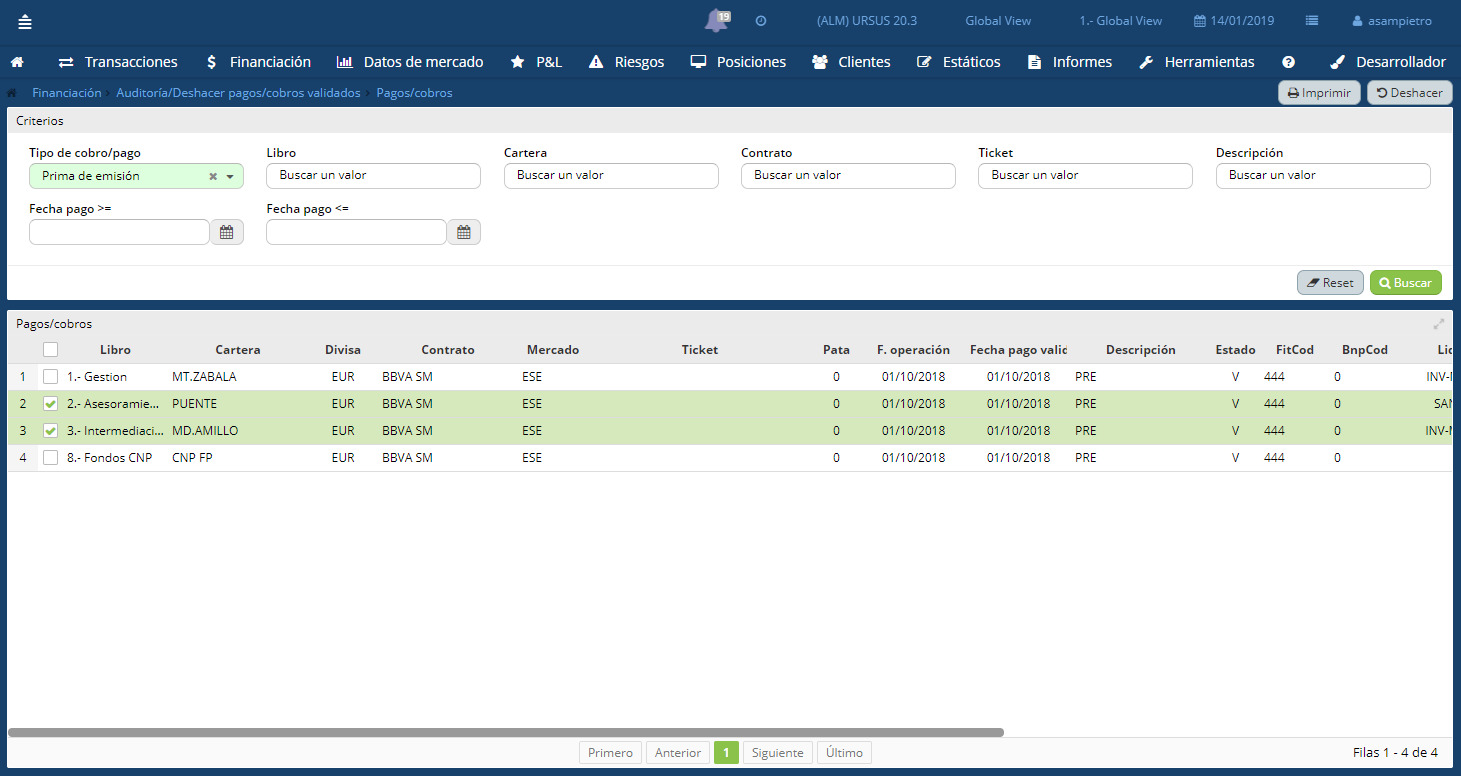
\includegraphics[width=\textwidth]{auditoria}
\caption{Ventana de pagos y cobros}
\end{figure}

El primer evento que se ha tratado ha sido la prima de asistencia, que se explicará a continuación.

\subsubsection{Primas de asistencia}
\subsubsection{Primas de emisión}
\subsubsection{Derechos de suscripción}
\subsection{Optimización de ventanas}



\end{document}
